%%%%(c) COPYRIGHT NOTICE%FOLDUP
%%%%(c)
%%%%(c)  This file is a portion of the source for the textbook
%%%%(c)
%%%%(c)    Numerical Methods Course Notes,
%%%%(c)    Copyright 2004-2010 by Steven E. Pav
%%%%(c)
%%%%(c)  See the file COPYING.txt for copying conditions
%%%%(c)
%%%%(c)%UNFOLD

%%throat clearing%FOLDUP
\typeout{-- derivatives.tex}
\typeout{-- N� 2004-2010 Steven E. Pav}
%UNFOLD

%%local commands%FOLDUP
%UNFOLD

\chapter{Approximating Derivatives}
\label{chap:apxDeriv}

%%%%%%%%%%%%%%%%%%%%%%%%%%%%%%%%%%%%%%%%%%%%%%%
\section{Finite Differences}%FOLDUP
\label{sec:fdderivs}
\depson{sec:taylors}{sec:fdderivs}

Suppose we have some blackbox function $f(x)$ and we wish to calculate $f'(x)$
at some given $x$.  Not surprisingly, we start with Taylor's theorem:
\[
f(x+h) = f(x) + f'(x)h + \half[f''(\xi)h^2].
\]
Rearranging we get
\[
f'(x) = \frac{f(x+h) - f(x)}{h} - \half[f''(\xi)h].
\]
Remember that $\xi$ is between $x$ and $x+h,$ but its exact value is not known.
If we wish to calculate $f'(x),$ we cannot evaluate $f''(\xi),$ so we
approximate the derivative by dropping the last term.
That is, we calculate $\Bracks{f(x+h) - f(x)}/h$ as an 
approximation\footnote{This approximation for $f'(x)$ should remind you of the
definition of $f'(x)$ as a limit.} to $f'(x).$ In so doing, we have dropped the
last term.  If there is a finite bound on $f''(z)$ on the interval in question
then the dropped term is bounded by a constant times $h.$  That is,
\begin{empheq}[box=\widefbox]{equation}
f'(x) = \frac{f(x+h) - f(x)}{h} + \bigo{h}
\label{eqn:fwddiff}
\end{empheq}

The error that we incur when we approximate $f'(x)$ by calculating $\Bracks{f(x+h) -
f(x)}/h$ is called \emph{truncation error}.\index{error!truncation}
It has nothing to do with the kind of error that you get when you
do calculations with a computer with limited precision; even if you worked in
infinite precision, you would still have truncation error.  

The truncation error can be made small by making $h$ small.  However, as $h$
gets smaller, precision will be lost in \eqnref{fwddiff} due to subtractive
cancellation.  The error in calculation for small $h$ is called \emph{roundoff
error}.\index{error!roundoff} Generally the roundoff error will increase as $h$
decreases.  Thus there is a nonzero $h$ for which the sum of these two errors
is minimized.  See \bkexpref{hdip} for an example of this.

The truncation error for this approximation is \bigo{h}.  
We may want a more precise approximation.  By now, you
should know that any calculation starts with Taylor's Theorem:
\begin{eqnarray*}
f(x+h) &=& f(x) + f'(x) h + \frac{f''(x)}{2} h^2 + \frac{f'''(\xi_1)}{3!} h^3\\
f(x-h) &=& f(x) - f'(x) h + \frac{f''(x)}{2} h^2 - \frac{f'''(\xi_2)}{3!} h^3
\end{eqnarray*}
By subtracting these two lines, we get 
\begin{eqnarray*}
f(x+h) - f(x-h) &=& 2 f'(x) h + \frac{f'''(\xi_1) + f'''(\xi_2)}{3!} h^3.
\end{eqnarray*}
Thus
\begin{eqnarray*}
2 f'(x) h &=& f(x+h) - f(x-h) - \frac{f'''(\xi_1) + f'''(\xi_2)}{3!} h^3\\
f'(x) &=& \frac{f(x+h) - f(x-h)}{2h} - \Bracks{\frac{f'''(\xi_1) +
f'''(\xi_2)}{2}} \frac{h^2}{6}
\end{eqnarray*}
If $f'''(x)$ is continuous, then there is some $\xi$ between $\xi_1,\xi_2$ such
that $f'''(\xi) = \frac{f'''(\xi_1) + f'''(\xi_2)}{2}.$  (This is the MVT at
work.) Assuming some uniform bound on $f'''(\cdot),$ we get

\begin{empheq}[box=\widefbox]{equation}
f'(x) = \frac{f(x+h) - f(x-h)}{2h} + \bigo{h^2}
\label{eqn:cendiff}
\end{empheq}

In some situations it may be necessary to use evaluations of a function at
``odd'' places to approximate a derivative.  These are usually straightforward
to derive, involving the use of Taylor's Theorem.  The following examples
illustrate:

\begin{bkexprob}%FOLDUP
Use evaluations of $f$ at $x+h$ and $x+2h$ to approximate $f'(x),$ assuming
$f(x)$ is an \emph{analytic} function, \ie one with infintely many derivatives.
\begin{bksolution}
First use Taylor's Theorem to expand $f(x+h)$ and $f(x+2h)$, then subtract to
get some factor of $f'(x)$:
\[
\begin{array}{rcl}
f(x+2h) &=& f(x) + 2h f'(x) + \frac{4 h^2}{2!} f''(x) +
				\frac{8 h^3}{3!} f'''(x) + \frac{16 h^4}{4!} f^{(4)}(x) + \ldots
				\vspace{1mm}\\
f(x+h) &=& f(x) + h f'(x) + \frac{h^2}{2!} f''(x) +
				\frac{h^3}{3!} f'''(x) + \frac{h^4}{4!} f^{(4)}(x) + \ldots
				\vspace{1mm}\\
\hline
\vspace{-4mm}& &\\
 f(x+2h) - f(x+h) &=& h f'(x) + \frac{3 h^2}{2!} f''(x) +
				\frac{7 h^3}{3!} f'''(x) + \frac{15 h^4}{4!} f^{(4)}(x) + \ldots
				\vspace{1mm}\\
\Parens{f(x+2h) - f(x+h)}/h &=& f'(x) + \frac{3 h}{2!} f''(x) +
				\frac{7 h^2}{3!} f'''(x) + \frac{15 h^3}{4!} f^{(4)}(x) + \ldots\\
\end{array}
\]
Thus
\(\Parens{f(x+2h) - f(x+h)}/h = f'(x) + \bigo{h}\)
\end{bksolution}
\end{bkexprob}%UNFOLD
\begin{bkexprob}%FOLDUP
Show that
\[\frac{4f(x+h) - f(x+2h) - 3f(x)}{2h} = f'(x) + \bigo{h^2},\]
for $f$ with sufficient number of derivatives
\begin{bksolution}
In this case we do not have to find the approximation scheme, it is given to
us.  We only have to expand the appropriate terms with Taylor's Theorem. As
before:
\[
\begin{array}{rcl}
f(x+h) &=& f(x) + h f'(x) + \frac{h^2}{2!} f''(x) +
				\frac{h^3}{3!} f'''(x) + \ldots
				\vspace{1mm}\\
4f(x+h) &=& 4f(x) + 4h f'(x) + \frac{4h^2}{2!} f''(x) +
				\frac{4h^3}{3!} f'''(x) + \ldots
				\vspace{1mm}\\
f(x+2h) &=& f(x) + 2h f'(x) + \frac{4 h^2}{2!} f''(x) +
				\frac{8 h^3}{3!} f'''(x) + \ldots
				\vspace{1mm}\\
\hline
\vspace{-4mm}& &\\
4 f(x+h) - f(x+2h) &=& 3 f(x) + 2h f'(x) + 0 f''(x) +
				\frac{-4 h^3}{3!} f'''(x) + \ldots
				\vspace{1mm}\\
4 f(x+h) - f(x+2h) - 3f(x) &=& 2h f'(x) + \frac{-4 h^3}{3!} f'''(x) + \ldots
				\vspace{1mm}\\
\Parens{4 f(x+h) - f(x+2h) - 3f(x)}/2h &=& f'(x) + \frac{-2 h^2}{3!} f'''(x) + \ldots
				\vspace{1mm}
\end{array}
\]
\end{bksolution}
\end{bkexprob}%UNFOLD

%%%%%%%%%%%%%%%%%%%%%%%%%%%%%%%%%%%%%%%%%%%%%%%
\subsection{Approximating the Second Derivative}%FOLDUP

Suppose we want to approximate the second derivative of some blackbox 
function $f(x)$.  Again, start with Taylor's Theorem:

\begin{eqnarray*}
f(x+h) &=& f(x) + f'(x) h + \frac{f''(x)}{2} h^2 + \frac{f'''(x)}{3!} h^3 
 + \frac{f^{(4)}(x)}{4!} h^4 + \ldots\\
f(x-h) &=& f(x) - f'(x) h + \frac{f''(x)}{2} h^2 - \frac{f'''(x)}{3!} h^3
 + \frac{f^{(4)}(x)}{4!} h^4 - \ldots 
\end{eqnarray*}

Now \emph{add} the two series to get
\begin{eqnarray*}
f(x+h) + f(x-h) &=& 2 f(x) + h^2{f''(x)} + 2 \frac{f^{(4)}(x)}{4!} h^4 + 
2 \frac{f^{(6)}(x)}{6!} h^6 + \ldots
\end{eqnarray*}

Then let
\begin{eqnarray*}
\psi(h) = \frac{f(x+h) - 2f(x) + f(x-h)}{h^2} &=& {f''(x)} + 2 \frac{f^{(4)}(x)}{4!} h^2 
	+ 2 \frac{f^{(6)}(x)}{6!} h^4 + \ldots,\\
	&=& f''(x) + \sum_{k=1}^{\infty} b_{2k} h^{2k}.
\end{eqnarray*}

Thus we can use Richardson Extrapolation on $\psi(h)$ to get higher order
approximations.

This derivation also gives us the \emph{centered difference} approximation to
the second derivative:\index{centered difference}
\begin{empheq}[box=\widefbox]{equation}
f''(x) = \frac{f(x+h) - 2f(x) + f(x-h)}{h^2} + \bigo{h^2}.
\label{eqn:twocendiff}
\end{empheq}
%UNFOLD
%UNFOLD
%%%%%%%%%%%%%%%%%%%%%%%%%%%%%%%%%%%%%%%%%%%%%%%
\section{Richardson Extrapolation}%FOLDUP
\label{sec:richardextrap}
\depson{sec:fdderivs}{sec:richardextrap}

The centered difference approximation gives a truncation error of $\bigo{h^2},$ which is better than
$\bigo{h}.$  Can we do better? %(Always ask yourself that.)
Let's define
\[\phi(h) = \oneby{2h}\Bracks{f(x+h) - f(x-h)}.\]

Had we expanded the Taylor's Series for $f(x+h),f(x-h)$ to more terms we would
have seen that
\begin{eqnarray*}
\phi(h) &=& f'(x) + a_2 h^2 + a_4 h^4 + a_6 h^6 + a_8 h^8 + \ldots
\end{eqnarray*}
The constants $a_i$ are a function of $f^{(i+1)}(x)$ only. (In fact, they should
take the value of $\frac{f^{(i+1)}(x)}{(i+1)!}$.)  What happens if we now calculate
$\phi(h/2)$? 
\begin{eqnarray*}
\phi(h/2) &=& f'(x) + \oneby{4} a_2 h^2 + \oneby{16} a_4 h^4 + \oneby{64} a_6
h^6 + \oneby{256} a_8 h^8 + \ldots
\end{eqnarray*}

But we can combine this with $\phi(h)$ to get better accuracy.  We have to be a
little tricky, but we can get the $\bigo{h^2}$ terms to cancel by taking the
right multiples of these two approximations:
\begin{eqnarray*}
\phi(h) - 4 \phi(h/2) &=& - 3 f'(x) + \frac{3}{4} 4 h^4 + \frac{15}{16} a_6 h^6
+ \frac{63}{64} a_8 h^8 + \ldots\\
\frac{4 \phi(h/2) - \phi(h)}{3} &=& f'(x) - \frac{1}{4} 4 h^4 - \frac{5}{16} a_6 h^6
- \frac{21}{64} a_8 h^8 + \ldots
\end{eqnarray*}
This approximation has a truncation error of $\bigo{h^4}.$ 

This technique of getting better approximations is known as the
\emph{Richardson Extrapolation}, and can be repeatedly applied.  We will also
use this technique later to get better quadrature rules--that is, ways of
approximating the definite integral of a function.
\index{Richardson Extrapolation}

%%%%%%%%%%%%%%%%%%%%%%%%%%%%%%%%%%%%%%%%%%%%%%%
\subsection{Abstracting Richardson's Method}%FOLDUP

We now discuss Richardson's Method in a more abstract framework.  Suppose you
want to calculate some quantity $L,$ and have found, through theory, some
approximation:
\[
\phi(h) = L + \sum_{k=1}^{\infty} a_{2k} h^{2k}.
\]
Let 
\[D(n,0) = \phi\Parens{\frac{h}{2^n}}.\]
Now define
\begin{empheq}[innerbox=\widefbox]{equation}
D(n,m) = \frac{4^m D(n,m-1) - D(n-1,m-1)}{4^m - 1}.
\label{eqn:richmethdef}
\end{empheq}

We will be interested in calculating $D(n,n)$ for some $n.$  We claim that 
\[D(n,n) = L + \bigo{h^{2(n+1)}}.\]

First we examine the recurrence for $D(n,m).$  As in divided differences, we
use a pyramid table:
\[\begin{array}{ccccc}
D(0,0) & & & & \\
D(1,0) & D(1,1) & & & \\
D(2,0) & D(2,1) & D(2,2) & & \\
\vdots & \vdots & \vdots & \ddots & \\
D(n,0) & D(n,1) & D(n,2) & \cdots & D(n,n)
\end{array}\]
By definition we know how to calculate the first column of this table;  every
other entry in the table depends on two other entries, one directly to the
left, and the other to the left and up one space.  Thus to calculate $D(n,n)$
we have to compute this whole lower triangular array.

We want to show that $D(n,n) = L + \bigo{h^{2(n+1)}},$ that is $D(n,n)$ is a 
\bigo{h^{2(n+1)}} approximation to $L$.  The following theorem gives this
result:

\begin{bktheorem}[Richardson Extrapolation]%FOLDUP
There are constants $a_{k,m}$ such that
\[D(n,m) = L + \sum_{k=m+1}^{\infty} a_{k,m} \Parens{\frac{h}{2^n}}^{2k} \qquad
\Parens{0\le m \le n}.\]
\end{bktheorem}%UNFOLD
The proof is by an easy, but tedious, induction.  We skip the proof.
%\begin{proof}%FOLDUP
%Our proof is by induction.  By definition of $D(n,0),$ and our assumptions on
%$\phi(h),$ the relation obviously holds for any $n$ and with $m=0.$  
%
%Now, given some $n,m$ assume the relation to be proven holds for $D(n-1,m-1),$
%and $D(n,m-1)$; we try to prove it for $D(n,m).$ This should be simple:
%
%\begin{eqnarray*}
%D(n,m) &=& \frac{4^m D(n,m-1) - D(n-1,m-1)}{4^m - 1}\\
% &=& \oneby{4^m -1} \Bracks{4^m L + 4^m \sum_{k=m}^\infty a_{k,m-1}
% \Parens{\frac{h}{2^n}}^{2k} - L - \sum_{k=m}^\infty a_{k,m-1}
% \Parens{\frac{h}{2^{n-1}}}^{2k}},\\
% &=& \oneby{4^m -1} \left[\Parens{4^m -1} L + 4^m a_{m,m-1}
% \Parens{\frac{h}{2^n}}^{2m} + 4^m \sum_{k=m+1}^\infty a_{k,m-1}
% \Parens{\frac{h}{2^n}}^{2k} \right.\\
% &=& \qquad \left. - a_{m,m-1} \Parens{\frac{h}{2^{n-1}}}^{2m} - 
% \sum_{k=m+1}^\infty a_{k,m-1} \Parens{\frac{h}{2^{n-1}}}^{2k} \right],\\
% &=& L + \oneby{4^m -1} \Bracks{4^m \sum_{k=m+1}^\infty a_{k,m-1}
% \Parens{\frac{h}{2^n}}^{2k} - \sum_{k=m+1}^\infty a_{k,m-1} \Parens{\frac{h}{2^{n-1}}}^{2k}},\\
% &=& L + \oneby{4^m -1} \Bracks{\sum_{k=m+1}^\infty 4^m a_{k,m-1}
% \Parens{\frac{h}{2^n}}^{2k} - \sum_{k=m+1}^\infty a_{k,m-1} 2^{2k} \Parens{\frac{h}{2^{n}}}^{2k}},\\
% &=& L + \sum_{k=m+1}^\infty \frac{4^m a_{k,m-1} - a_{k,m-1} 2^{2k}}{4^m -1} \Parens{\frac{h}{2^{n}}}^{2k},\\
%D(n,m) &=& L + \sum_{k=m+1}^\infty a_{k,m} \Parens{\frac{h}{2^{n}}}^{2k}.
%\end{eqnarray*}
%For the properly defined $a_{k,m}.$ 
%\end{proof}%UNFOLD
%%UNFOLD
%%%%%%%%%%%%%%%%%%%%%%%%%%%%%%%%%%%%%%%%%%%%%%%
\subsection{Using Richardson Extrapolation}%FOLDUP

We now try out the technique on an example or two.

\begin{bkexprob}%FOLDUP
Approximate the derivative of $f(x) = \log x$ at $x=1.$
\begin{bksolution}
The real answer is $f'(1) = 1/1 = 1,$ but our computer doesn't know that.
Define
\[\phi(h) = \oneby{2h}\Bracks{f(1+h) - f(1-h)} = \frac{\log \frac{1+h}{1-h}}{2h}.\]
Let's use $h=0.1$.  We now try to find $D(2,2),$ which is supposed to be a
\bigo{h^6} approximation to $f'(1) = 1$:
%\approx \frac{ 4 (1.000834586) - 1.003353477}{3} 
\[\begin{array}{c||c|c|c}
n \backslash m & 0 & 1 & 2\\
\hline
\hline
0 & \frac{\log \frac{1.1}{0.9}}{0.2} \approx 1.003353477 & &  \\
\hline
1 & \frac{\log \frac{1.05}{0.95}}{0.1} \approx 1.000834586 & 
\approx 0.999994954 &  \\
\hline
2 & \frac{\log \frac{1.025}{0.975}}{0.05} \approx 1.000208411 & \approx
0.999999686 & \approx 1.000000002
\end{array}\]

This shows that the Richardson method is pretty good.  However, notice that for
this simple example, we have, already, that $\phi(0.00001) \approx
0.999999999$.
\end{bksolution}
\end{bkexprob}%UNFOLD
\begin{bkexprob}\label{bkexp:hdip}%FOLDUP
Consider the ugly function:
\[f(x) = \arctan(x).\]
Attempt to find $f'(\sqrt{2}).$  Recall that $f'(x) = \oneby{1+x^2},$ so the
value that we are seeking is \oneby{3}.
\begin{bksolution}
Let's use $h=0.01$.  We now try to find $D(2,2),$ which is supposed to be a
\bigo{h^6} approximation to $\oneby{3}$:
\[\begin{array}{c||c|c|c}
n \backslash m & 0 & 1 & 2 \\
\hline
\hline
0 & 0.333339506181068 & & \\
\hline
1 & 0.333334876543723 & 0.333333333331274 & \\
\hline
2 & 0.33333371913582 & 0.333333333333186 & 0.333333333333313 \\
\hline
\end{array}\]
%\[\begin{array}{c||c|c|c|c}
%n \backslash m & 0 & 1 & 2 & 3\\
%\hline
%\hline
%0 & 0.333339506181068 & & & \\
%\hline
%1 & 0.333334876543723 & 0.333333333331274 & & \\
%\hline
%2 & 0.33333371913582 & 0.333333333333186 & 0.333333333333313 & \\
%\hline
%3 & 0.333333429783966 & 0.333333333333348 & 0.333333333333359 & 0.33333333333336 \\
%\end{array}\]

Note that we have some motivation to use Richardson's method in this case:
If we let
\[\phi(h) = \oneby{2h}\Bracks{f(\sqrt{2}+h) - f(\sqrt{2}-h)},\]
then making $h$ small gives a good approximation to $f'\Parens{\sqrt{2}}$
\emph{until subtractive cancelling takes over}.  The following table
illustrates this:

\[\begin{array}{c|c}
h & \phi(h)\\
\hline
\hline
1.0 & 0.39269908169872408 \\
0.1 & 0.33395069677431943 \\
0.01 & 0.33333950618106845 \\
0.001 & 0.33333339506169679 \\
0.0001 & 0.33333333395058062 \\
\tenex{1}{-5} & 0.33333333334106813 \\
\tenex{1}{-6} & 0.33333333332441484 \\
\tenex{1}{-7} & 0.33333333315788138 \\
\tenex{1}{-8} & 0.33333332760676626 \\
\tenex{1}{-9} & 0.33333336091345694 \\
\tenex{1}{-10} & 0.333333360913457 \\
\tenex{1}{-11} & 0.333333360913457 \\
\tenex{1}{-12} & 0.33339997429493451 \\
\tenex{1}{-13} & 0.33306690738754696 \\
\tenex{1}{-14} & 0.33306690738754696 \\
\tenex{1}{-15} & 0.33306690738754691 \\
\tenex{1}{-16} &         0 
\end{array}\]

The data are illustrated in \figref{hdip}.
Notice that $\phi(h)$ gives at most 10 decimal places of accuracy, then begins
to deteriorate;  Note however, we get 13 decimal places from $D(2,2).$
%\figref{hdip}%FOLDUP
\begin{figure}[htb!]
\centering
	\psfrag{hdip}[Br][r][0.8]{total error}
	\includegraphics[width=0.60\columnwidth,angle=270,clip=]{hdip.eps}
\caption{The total error for the centered difference approximation to
$f'(\sqrt{2})$ is shown versus $h.$  The total error is the sum of a truncation
term which decreases as $h$ decreases, and a roundoff term which increases.
The optimal $h$ value is around \tenex{1}{-5}.  Note that Richardson's $D(2,2)$
approximation with $h=0.01$ gives much better results than this optimal $h.$}\label{fig:hdip}
\end{figure}%UNFOLD
\end{bksolution}
\end{bkexprob}%UNFOLD
%\begin{bkexample}%FOLDUP
%Consider the really ugly function:
%\[f(x) = (x/0.0001)*\arctan(x/0.0001) - 0.5 \log \Parens{1 +
%\Parens{\frac{x}{0.0001}}^2}.\]
%This function has the funny property that 
%\[f'(x) = \oneby{0.0001}\arctan(x/0.0001).\]
%And thus $f'(0) = 0.$  Let's see how well Richardson's method does.
%
%
%
%
%Approximate the derivative of $f(x) = \log x$ at $x=1.$
%\\The real answer is $f'(1) = 1/1 = 1,$ but our computer doesn't know that.
%Define
%\[\phi(h) = \oneby{2h}\Bracks{f(1+h) - f(1-h)} = \frac{\log \frac{1+h}{1-h}}{2h}.\]
%Let's use $h=0.1$.  We now try to find $D(2,2),$ which is supposed to be a
%\bigo{h^6} approximation to $f'(1) = 1$:
%%\approx \frac{ 4 (1.000834586) - 1.003353477}{3} 
%\[\begin{array}{c||c|c|c}
%n \backslash m & 0 & 1 & 2\\
%\hline
%\hline
%0 & \frac{\log \frac{1.1}{0.9}}{0.2} \approx 1.003353477 & &  \\
%\hline
%1 & \frac{\log \frac{1.05}{0.95}}{0.1} \approx 1.000834586 & 
%\approx 0.999994954 &  \\
%\hline
%2 & \frac{\log \frac{1.025}{0.975}}{0.05} \approx 1.000208411 & \approx
%0.999999686 & \approx 1.000000002
%\end{array}\]
%
%This shows that the Richardson method is pretty good.  However, notice that for
%this simple example, we have, already, that $\phi(0.00001) \approx
%0.999999999$.
%
%\end{bkexample}%UNFOLD
%UNFOLD
%UNFOLD
%%%%%%%%%%%%%%%%%%%%%%%%%%%%%%%%%%%%%%%%%%%%%%%
%\section{Exercises}%FOLDUP
\begin{bkexs}

%%%%%%%%%%%%%%%%%% 
\item Derive the approximation
\[f'(x) \approx \frac{4f(x+h) - 3f(x) - f(x-2h)}{6h}\]
using Taylor's Theorem.  


\begin{compactenum}
\item Assuming that $f(x)$ has bounded derivatives, give the accuracy of the
above approximation.  Your answer should be something like $\bigo{h^{?}}$.
\item Let $f(x) = x^3.$  Approximate $f'(0)$ with this approximation, using
$h=\oneby{4}.$
\end{compactenum}

%%%%%%%%%%%%%%%%%% 
\item Let $f(x)$ be an \emph{analytic} function, \ie one which is infinitely
differentiable.  Let $\psi(h)$ be the centered difference approximation to the
first derivative:
\[
\psi(h) = \frac{f(x+h) - f(x-h)}{2h}
\]

\begin{compactenum}
\item Show that \(\psi(h) = f'(x) + \frac{h^2}{3!}f'''(x) + 
	\frac{h^4}{5!}f^{(5)}(x) + 
	\frac{h^6}{7!}f^{(7)}(x) + \ldots
\)
\item Show that \[\frac{8 \Parens{\psi(h) - \psi(h/2)}}{h^2} = f'''(x) +
\bigo{h^2}.\]
\end{compactenum}

%%%%%%%%%%%%%%%%%% 
\item Derive the approximation
\[f'(x) \approx \frac{4f(x+3h) +5f(x) - 9f(x-2h)}{30h}\]
using Taylor's Theorem.  
\begin{compactenum}[(a)]
	\item What order approximation is this? (Assume $f(x)$ has
	bounded derivatives of arbitrary order.)
	\item Use this formula to approximate $f'(0),$ where $f(x) = x^4,$ and
	$h=0.1$
\end{compactenum}

%%%%%%%%%%%%%%%%%% 
\item Suppose you want to know quantity $Q,$ and can approximate it with some
formula, say $\phi(h),$ which depends on parameter $h$, and such that 
$\phi(h) = Q + a_1 h + a_2 h^2 + a_3 h^3 + a_4 h^4 + \ldots$
Find some linear combination of $\phi(h)$ and $\phi(-h)$ which is a \bigo{h^2}
approximation to $Q.$
%%%%%%%%%%%%%%%%%% 
\item Assuming that $\phi(h) = Q + a_2 h^2 + a_4 h^4 + a_6 h^6 \ldots$,
find some combination of $\phi(h), \phi(h/3)$ which is a \bigo{h^4}
approximation to $Q.$
%%%%%%%%%%%%%%%%%% 
\item Let $\lambda$ be some number in \ooinv{0}{1}.  
Assuming that $\phi(h) = Q + a_2 h^2 + a_4 h^4 + a_6 h^6 \ldots$,
find some combination of $\phi(h), \phi(\lambda h)$ which is a \bigo{h^4}
approximation to $Q.$  To make the constant associated with the $h^4$ term
small in magnitude, what should you do with $\lambda$?  Is this practical?
Note that the method of Richardson Extrapolation that we considered used the
value $\lambda = 1/2$.

%%%%%%%%%%%%%%%%%% 
\item
Assuming that $\phi(h) = Q + a_2 h^2 + a_4 h^4 + a_6 h^6 \ldots$,
find some combination of $\phi(h), \phi(h/4)$ which is a \bigo{h^4}
approximation to $Q.$
%%%%%%%%%%%%%%%%%% 
\item
Suppose you have some great computational approximation to the quantity $Q$
such that
$\psi(h) = Q + a_3 h^3 + a_6 h^6 + a_9 h^9 \ldots$
Can you find some combination of $\psi(h), \psi(h/2)$ which is a \bigo{h^6}
approximation to $Q?$


%%%%%%%%%%%%%%%%%% 
\item Complete the following Richardson's Extrapolation Table, assuming the
first column consists of values $D(n,0)$ for $n=0,1,2$:
\[\begin{array}{c||c|c|c}
n \backslash m & 0 & 1 & 2 \\
\hline
\hline
0 & 2 & & \\
\hline
1 & 1.5 & ? & \\
\hline
2 & 1.25 & ? & ? \\
\hline
\end{array}\]
(See \eqnref{richmethdef} if you've forgotten the definitions.)

%%%%%%%%%%%%%%%%%% 
\item Write code to complete a Richardson's Method table, given the first
column.  
Your m-file should have header line like:
\begin{verbatim}
function Dnn = richardsons(col0)
\end{verbatim}
where \texttt{Dnn} is the value at the lower left corner of the table, $D(n,n)$
while \texttt{col0} is the column of $n+1$ values $D(i,0),$ for
$i=\zerotox{n}.$
Test your code on the following input:
\begin{verbatim}
octave:1> col0 = [1 0.5 0.25 0.125 0.0625 0.03125];
octave:2> richardsons(col0)
ans = 0.019042
\end{verbatim}
\begin{compactenum}
	\item What do you get when you try the following?
	\begin{verbatim}
	octave:5> col0 = [1.5 0.5 1.5 0.5 1.5 0.5 1.5];
	octave:6> richardsons(col0)
	\end{verbatim}
	%ans = 1.9845
	\item What do you get when you try the following?
	\begin{verbatim}
	octave:7> col0 = [0.9 0.99 0.999 0.9999 0.99999];
	octave:8> richardsons(col0)
	\end{verbatim}
	%ans = 1.0000
\end{compactenum}


\end{bkexs}
%UNFOLD
%for vim modeline: (do not edit)
% vim:ts=2:sw=2:tw=79:fdm=marker:fmr=FOLDUP,UNFOLD:cms=%%s:tags=tags;:syntax=tex:filetype=tex:ai:si:cin:nu:fo=croqt:cino=p0t0c5(0:
